\setcounter{section}{94}
\section{Определение изоморфизма графов. Алгоритм проверки изоморфности двух ориентированных или неориентированных деревьев за O(n log n).}

\begin{figure}[!htb]
   \begin{minipage}{.5\textwidth}
     \centering
     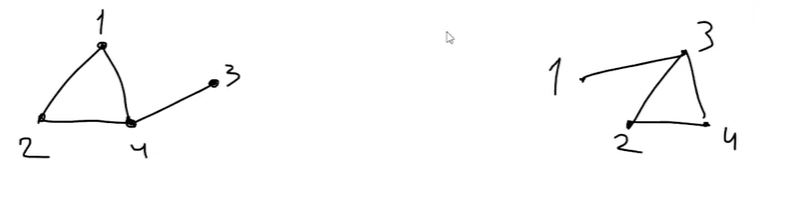
\includegraphics[height = 1.5 cm]{images/95_isomorphism}
     % \includegraphics[width=.7\linewidth]{95_example-image-a}%
     \caption{Пример изоморфизма.}
   \end{minipage}\hfill
    \begin{minipage}{.5\textwidth}
     \centering
     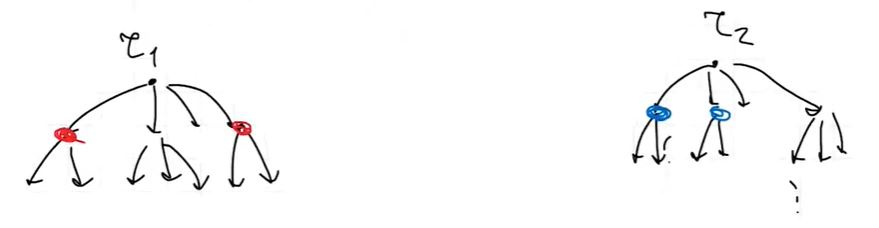
\includegraphics[height = 1.5 cm]{images/95_isomorph2}
     \caption{Изоморфизм ориентированных деревьев.}
   \end{minipage}
\end{figure}

Пусть G и H - два неориентированных графа. Функция $\varphi: V(G) \rightarrow V(H)$ - \textbf{изоморфизм}, если:

1) $\varphi$ - биекция

2) $(u, v) \in E(G) \Leftrightarrow (\varphi(u), \varphi(v)) \in E(V)$

\textit{Замечание}. Для ориентированных аналогично. \\

\textbf{Пункт 1}. Проверка ориентированных (подвешенных/корневых) деревьев на изоморфность. 

0. См. рис. 2 - совсем тривиальный алгоритм, сравнивающий по количеству сыновей, не совсем работает, валится на совпадениях по количеству. 

1. Пусть G - корневое дерево с корнем в r. Тогда для всех поддеревьев найдём "номер класса эквивалентности": мы разбиваем вершины на классы эквивалентности по количеству детей в каждом из поддеревьев, которые являются их сыновьями. Получаются вектора размеров поддеревьев, и по их равенству (без учёта порядка элементов в векторе, скажем, эл-ты отсортированы) вводятся классы эквивалентности.


\lstinputlisting[language=C++, emph={int,char,double,float,unsigned,vector,<,>,map}, emphstyle={\color{blue}} ]{code/95_isomorph1.cpp}

3. Для двух деревьев - запускаем dfs[$r_1$], dfs[$r_2$], после чего сравниваем classes. 

Де-факто это быстро, хотя точную асимптотику сказать сложно (мап работает за логарифм длины сравнения, а там сравниваются вектора; но с хешированием векторов можно ускорить, если надо, и тогда будет $O(n)$ - время работы хеш-таблицы.)

\textbf{Пункт 2}. Проверка неориентированных деревьев на изоморфность: раньше у нас были фиксированные пары корней, которые мы сопоставляли: в биекции корень всегда сопоставляется корню - тут же мы берём пару центроидов (все возможные пары центроидов), потому что аналогично, центроид в первом графе останется центроидом во втором, вот наша гарантированная пара, а дальше - пункт 1. 